\documentclass[a4paper,12pt]{article}
\usepackage{a4wide}
\usepackage[utf8]{inputenc}
\usepackage[english]{babel}
\usepackage{hyperref}
\usepackage{graphicx}
\usepackage{epstopdf}
\usepackage{subcaption}
\usepackage{amssymb}


%\usepackage[labelformat=empty]{caption}
\usepackage{float}
%opening
\title{D7017E:\@ Report}

\begin{document}
\author{  \\ Luleå Tekniska Universitet\\ 
971 87 Luleå, Sverige\\  
\\ Niklas Fuks
\\ Tim Granström 
\\ Nils Fitinghoff 
\\ Mikael Hedkvist 
\\ David Sandström 
\\ Anton Jerhamre
\\ Christopher Rosenvall
\\ Fredrik Bostrand 
\\ Henrik Nilsson Harnert 
\\ Axel Sundbom 
\\ Rickard Nordlander 
\\ Anders Mikkelä 
\\ Axel Vallin
\\ Linn Danielsson
\\ Tobias Axelsson
}
\maketitle
\thispagestyle{empty}
\newpage
\thispagestyle{empty}  
 \setcounter{page}{1}
\newpage
\thispagestyle{empty}  
 \begin{abstract}
Abstract
 \end{abstract}
\newpage

\tableofcontents{}
\thispagestyle{empty}
 \setcounter{page}{2}
 
 \newpage
 \setcounter{page}{3}

\section{Introduction}
\subsection{Background} 
At several studying programs at Luleå university of Technology, programming is a major part of the courses. Students may sometimes have some difficulty to know if they have programmed correctly until a lab supervisor controls the code written by the student. This may sometimes lead to long feedback time and the thoughts about the specific programming problems are forgotten between the feedback time. To increase the feedback time and make the programming more fun a platform for coding practice would be suitable. There are a lot of different applications on the internet but none are suitable enough for teachers and students at Luleå university of Technology. Gamification is shown to increase the activity of people, so why shouldn't gamification be suitable for programming? 

With direct feedback and with notable progress students may think that programming will be more fun. By small increments in the programming problem difficulty it's easier to succeed to the next step instead of having a large problem covering a lot of different syntax. With different difficulties every student can feel that they are challenged and receives rewards immediately. In different existing online tools it is possible for teachers to write exercises and tests where students then can solve and get feedback. 

But none of the tools found support that teachers can write exercises and have the gamification parts, they only support one of them. Many of the existing tools are complicated for teachers to implement in existing courses so it need to be simplified more for the teachers to use the platform otherwise it will not be used. The bottleneck concluded is the teachers mentioned above, they need to easily and in a few hours be able to implement a course in the platform. To fill this absence of information, interviews were conducted with teachers, students and finally a workshop was setup with teachers to try to broaden the picture of what is missing and what they need.


\subsection{Goals}   
The goal of the project was to find a teaching method for the students that facilitates learning for both basic and advanced programming by using gamification theories.
\\ \\
The purpose of gamification is to take elements from games and apply them in other areas to create an increased commitment within the applied area.
The target group is mainly students studying at Department of Computer Science, Electrical and Space Engineering  with a programming direction but also other educations within LTU that contain programming parts, for example teacher education where programming will become a central part in the future because of a revised curriculum for elementary school and high school that passed in the fall of 2017.
\\ \\
To reach the goal of the project, a platform that embodied these ideas was needed.
The goal was to have a platform that was easy for both users and teachers alike. Gamification was a big part of the platform but a realization that not all teachers wanted to use these elements was reached and because of this it needed to be simple to activate and disable gamification features for courses as the teacher saw fit. As such, a big goal during the development of the platform was to make features very modular.

\subsection{Expected result / requirements}  
The expected result was to deliver a web-based platform for learning programming. The platform should include gamification methods that stimulates the student so that they want to program more and be better at programming. The students should be able to write their code in the browser and then be able to validate if they have the correct outcome of the assignment. The platform should support progress and different levels so that every student is challenged. The platform shouldn't be limited to LTU even though LTU is the primary source that will use the platform. 

\subsubsection{Initial requirements} 
 \begin{itemize}
\item Full solution for writing and testing code.
\item Immediate feedback.
\item Show progress/statistics.
\item Involve gamification.
\item Support multiple programming language.
\item Teachers should be able to construct assignments.
\item Easy navigation.
\item Log in by CAS. 
\item Primary target is LTU students.
 \end{itemize}


\section{Working methods}
\subsection{Sprints} 
Agile work flow was used during the project. This was done by dividing the weeks into sprints. A sprint was expected to be one week but sometimes sprints become longer due to heavy workload. Every sprint was planed before the current sprint was ended. The group leaders planned the sprints, one from each current sub group along with the project leader. Taiga.io, a sprint planning tool kept track of the backlog and different task assigned to individual group members. This showed which task was completed and which needed to be helped with. During the project some of the members evaluated the tool Taiga.io and found that it could have been better if it was possible to add tasks to more than one person, if it was easier to assign points to a task and move a task to other sprints. A decision was made to keep Taiga.io because the members had gained experience with it and it would be impractical to split the backlog to a new tool.

\subsection{Groups} 
All of the different task sections were split into groups. During the project it was laborated on how many number of groups would be the most efficient for the project. The working model that was found was to have three groups with 4-5 members each as long as there were enough tasks in different sections for three groups. Every week at least one time all members met and discussed the previous week and the upcoming week. This became a meeting with 15 people that ended up talking over each other which felt ineffective. This was solved by minimizing the meeting members to three-four people: the project leader along with one group leader each from the frontend, backend and tester group. The leaders were democratically chosen in each active group and their task was to tell the other group leaders what they have and will accomplish during next period. They then went to their own groups and told them about the meeting. This worked well during the first weeks but less and less information were distributed to the group member as time went by. When this problem was then identified it was to short time left on the project to change the meeting method and instead it was simply decided that everyone needed to try and keep the quality of the distributed information up like it was in the first few weeks. \\
The different groups that has been presented are:\\
 \begin{itemize}
 \item Interviews
 \item Workshop
 \item Platform
 \item Theory
 \item Frontend
 \item Backend
 \item Tester.
 \end{itemize}


\subsection{Roles} 
All the project members had a responsibility that the project should succeed and it was important to contribute to the extent that each member was capable of.\\
The three major roles have been assigned during the project, these are \\
\textbf{Project leader} - Niklas Fuks which had an overview of the project and its sub tasks. Planned the meetings, sprints and held presentations with demos. \\
\textbf{Groupleader and software engineers} -\\
Axel Sundbom (tester)\\
Tobias Axelsson (backend) \\
Axel Vallin (frontend) \\
\textbf{Software engineers} -\\
Linn Danielsson\\
Nils Fitinghoff\\
Mikael Hedkvist\\
David Sandström\\
Anton Jerhamre\\
Christopher Rosenvall\\
Fredrik Bostrand\\
Henrik Nilsson Harnet\\
Tim Granström\\
Rickard Nordlander\\
Anders Mikkelä\\


\section{Prestudy} 
Since the goal of the project is a platform that can increase learning using gamification it was need to conduct a study about which parts of gamification is relevant for the platform and how should they be represented. Peter Parnes, the project owner suggested that the information could be collected by reading literature, having a workshop with teachers at LTU and some teachers outside the university and by interviewing a few teachers teaching in courses that could have use for the platform as a part of their course. An investigation was done about what tools and existing platforms are already available and if they could be reused and built on. This investigation was done by the platform group.

\subsection{Interviews}
The interviews were done by interviewing a couple of teachers teaching in courses at LTU. A group of four members set up individual meetings with each respective teacher where they asked relevant questions regarding a gamified coding platform. The most comprehensive and general questions during the interviews can be found in appendix, see section~\ref{Interview:questions}. The interview answers from the teachers were summarized to identify the most important elements that could be used. The most important elements were those which were repeated during several interviews and those that the interview group found most interesting. The identified and summarized elements are:

 \begin{itemize}
 \item Mandatory assignments would increase the participation frequency but would be less fun.
 \item Public scoreboard may be demotivating.
 \item Best result could be displayed in by a score.
 \item A balance between school and fun.
 \item Levels / different difficulties. 
 \item Even the weaker students should have a chance to solve assignments on the easier levels.
 \item No points or badges.
 \item Anonymous questions.
 \item Good for the lower grades.
 \item Must be easy to adapt the system into a course.
 \end{itemize}
These summarized answers was a good starting point to see which parts should be included later on in the platform and which parts should be excluded. 

\subsection{Platform}   
To meet the requirements and goals of the project it was clear that a platform that could compile and verify code was needed.
When the project started, the project owner had suggested tech.io which is a collaborative platform to share coding assignments through open-source ``playgrounds''. At a first glance, the platform seemed to match the needs of the project, but it was unsure if the platform would have an open API which the project communicate and work with. The developers of tech.io, CodinGame was contacted to find out if they would be open to sharing their API.

%Fyll ut med några av problemen vi identifierade med tech.io som vi skulle ha behövt lösa om vi hade använt det. (finns i wikin)

While waiting for an answer from tech.io, an investigation into alternative platforms to tech.io was launched and after some time of searching for a suitable alternative over the internet it was concluded that no platform found really matched the requirements that were set.

After waiting for several days, tech.io finally responded where they mentioned the possibility of using ``code snippets'' to embed coding assignments onto other sites than on tech.io, but they were evasive with the question if they would make their API open and never really answered this. After some time of consideration, a decision to not use tech.io was made because of the risk of becoming too dependent on their platform.

Because of this, creating a code verification platform/API from scratch was considered. While discussing about making a code verification platform from scratch, a new alternative was brought into light. A computer science student at LTU was currently creating a platform named Sockr for code verification and once again, it was considered to use a third party platform.

After some discussions with the student, he explained that he would be open for the project to use Sockr. A thorough investigation of the Sockr source code was however needed to make sure that it was actually useful for the project. When diving deeper into the source code of Sockr it became clear that once again, the project would not be able to use this in a good and sustainable way. While Sockr did have the functionality that the project needed, the source code was mostly undocumented, didn't have a clear API and the backend and frontend were too tightly coupled to be used in a sustainable way.

As such, after much research it was concluded that the best and most sustainable thing for the project would be to develop a code verification/compilation platform from scratch, effectively making the project completely independent of other services.


\subsection{Theory} 
A theory study was conducted where the task was to find what articles and the books have learned about gamification. A group with a couple of members sat down and read books and articles mostly found on internet. The group found a number of useful elements from gamification theory that could possibly be implemented into the platform, it was however realized that not all these elements could be implemented all at once and it was later needed to identify which elements who would gain priority. The elements that the theory group found useful were:
\begin{itemize}
\item Reward
\begin{itemize}
 \item Reward should give positive information since it increases the motivation.
 \item Rewards of controlling type is demotivating.
 \item If rewards ends it may be demotivating later on.
 \item Customization, collect points and be able to spend them.
 \end{itemize}
\item Progress
\begin{itemize}
    \item Progress should be in increasing order.
    \item Be careful with which moments should be graded.
    \item Large numbers are better.
    \item Bonus for overachieving. 
\end{itemize}
\item Freedom
\begin{itemize}
    \item Freely choose between assignments.
    \item Possibility to redo assignments.
\end{itemize}
\item Game mechanics
\begin{itemize}
    \item Chance?
    \item Duels?
    \item Take turns?
\end{itemize}
\item Leaderboard
\begin{itemize}
    \item Anonymous leaderboard.
    \item No disincentive
    \item No ranking, demotivated to have low rank
    \item Populate the leaderboard with fake users
\end{itemize}
\end{itemize}

\subsection{Comparison interviews and theory} 
To find the key aspects of gamification from both interviews and theory a comparison was made where a group compiled the data from the previous received feedback and other notes collected into a new list that could act as a basis for future decisions about gamification.
When compiling the list it was also important to take into account what parts that could actually be implemented during the project and which ones could be possible future work.
The newly formed list contained the following key elements:
\begin{itemize}
\item A lot of small assignments
\begin{itemize}
 \item A lot of structure, easy to understand the feedback.
 \item Levels.
\end{itemize}
\item Progress
\begin{itemize}
 \item Progress in increasing direction.
\end{itemize}
\item Freedom
\begin{itemize}
 \item The mandatory assignments have highest participation but may be demotivating.
 \item Students should have different options to solve a moment.
 \item Deadlines may be demotivating but also sometimes necessary.
 \item Redo an assignment multiple times.
\end{itemize}
\item Rewards
\begin{itemize}
 \item Should act as a positive information about the student skill level.
 \item Rewards should not act as a controlling factor.
 \item Redeemable points, e.g.\ avatars.
\end{itemize}
\item Feedback
\begin{itemize}
 \item Teachers should be able to check if students have understood the assignment or not.
\end{itemize}
\item Leaderboard
\begin{itemize}
 \item Divided opinions about how good leaderboards are.
 \item Anonymous leaderboards.
 \item Fake users so that no one is last.
\end{itemize}
\end{itemize}


\subsection{Workshop} 
A workshop was presented as an idea from the project owner Parnes as a way to find out how different teachers think that the system would look like and what features they feel should be included. A group of five people started to work by writing different scenarios for the workshop, see section~\ref{Worskshop:senarios}. As a preparation for the real workshop, these scenarios were then tested on a few members of the project group where the members were acting as teachers and they had to implement the planned workshop scenarios. This gave the workshop group some thoughts about what could be improved before the ordinary workshop with the teachers. 
The workshop with the teachers was made by splitting the teachers into two different groups and then they had 10--15 minutes to discuss the scenarios in the group and then another 10 minutes for discussions with the other group. 
The first scenario task was to discuss which type of system and elements could be available that would have motivated them as students. In the scenario 2 the groups had to imagine themselves being the examiners of a course and the groups got to discuss which limitations should be done in the system but also once again, how they could motivate their students. During the scenario 3 the task was to focus on embodying the ideas and thoughts from scenario 1 and 2 into an e-tool and how the general design should for said tool look like. A compiled list from both groups together from what was discussed and concluded during the workshop:
\\
Result from scenario 1
\begin{itemize}
\item Let assignments interlink.
\item Be able to choose which assignments should be done.
    \begin{itemize}
    \item Hard to grade, every goal of the course need to be met.
    \item Assignments with similar content.
    \end{itemize}
\item Constructive alignment, how goals, assignments and examination interacts.
\item Early and quick feedback.
\item Formative assessment, continuous feedback.
\item Groups assignments, hide the personal result.
\item AI Avatar that gives feedback.
\item Lot of visualization of the result.
\item Present the purpose of the assignment.
\item Different angle of the design depending on the user which is solving the assignment.
\end{itemize}

Result from scenario 2
\begin{itemize}
\item Not everything in a course should be change at same time.
\begin{itemize}
\item Old assignments could be divided.
\item Shorter feedback loop.
\item old assignments with new contex.
\end{itemize}
\item Updating the course introduction is cheap and makes the goals of the course more clear.
\item When the knowledge should be testes.
\begin{itemize}
\item Thoroughly, min/max, median or average.
\item In the end there is a written exam.
\end{itemize}
\item Invoke from elder students.
\item Peer-to-peer feedback.
\item Test one implementation even if it's bad.
\item Students creates assignments to each other.
\end{itemize}

Result from scenario 3
\begin{itemize}
\item Anonymous questions live
\begin{itemize}
\item ``Did you understand what I said?''
\item Directly feedback.
\end{itemize}
\item Direct chat, students and teacher.
\item Auto generated feedback to the teacher.
\begin{itemize}
\item Aggregate data from relevant measurements.
\end{itemize}
\item A student knowledge bank.
\begin{itemize}
\item Wiki.
\end{itemize}
\item Code correction / evaluation.
\end{itemize}


\begin{figure}[H]
  \centering
  \begin{minipage}[b]{0.7\textwidth}
    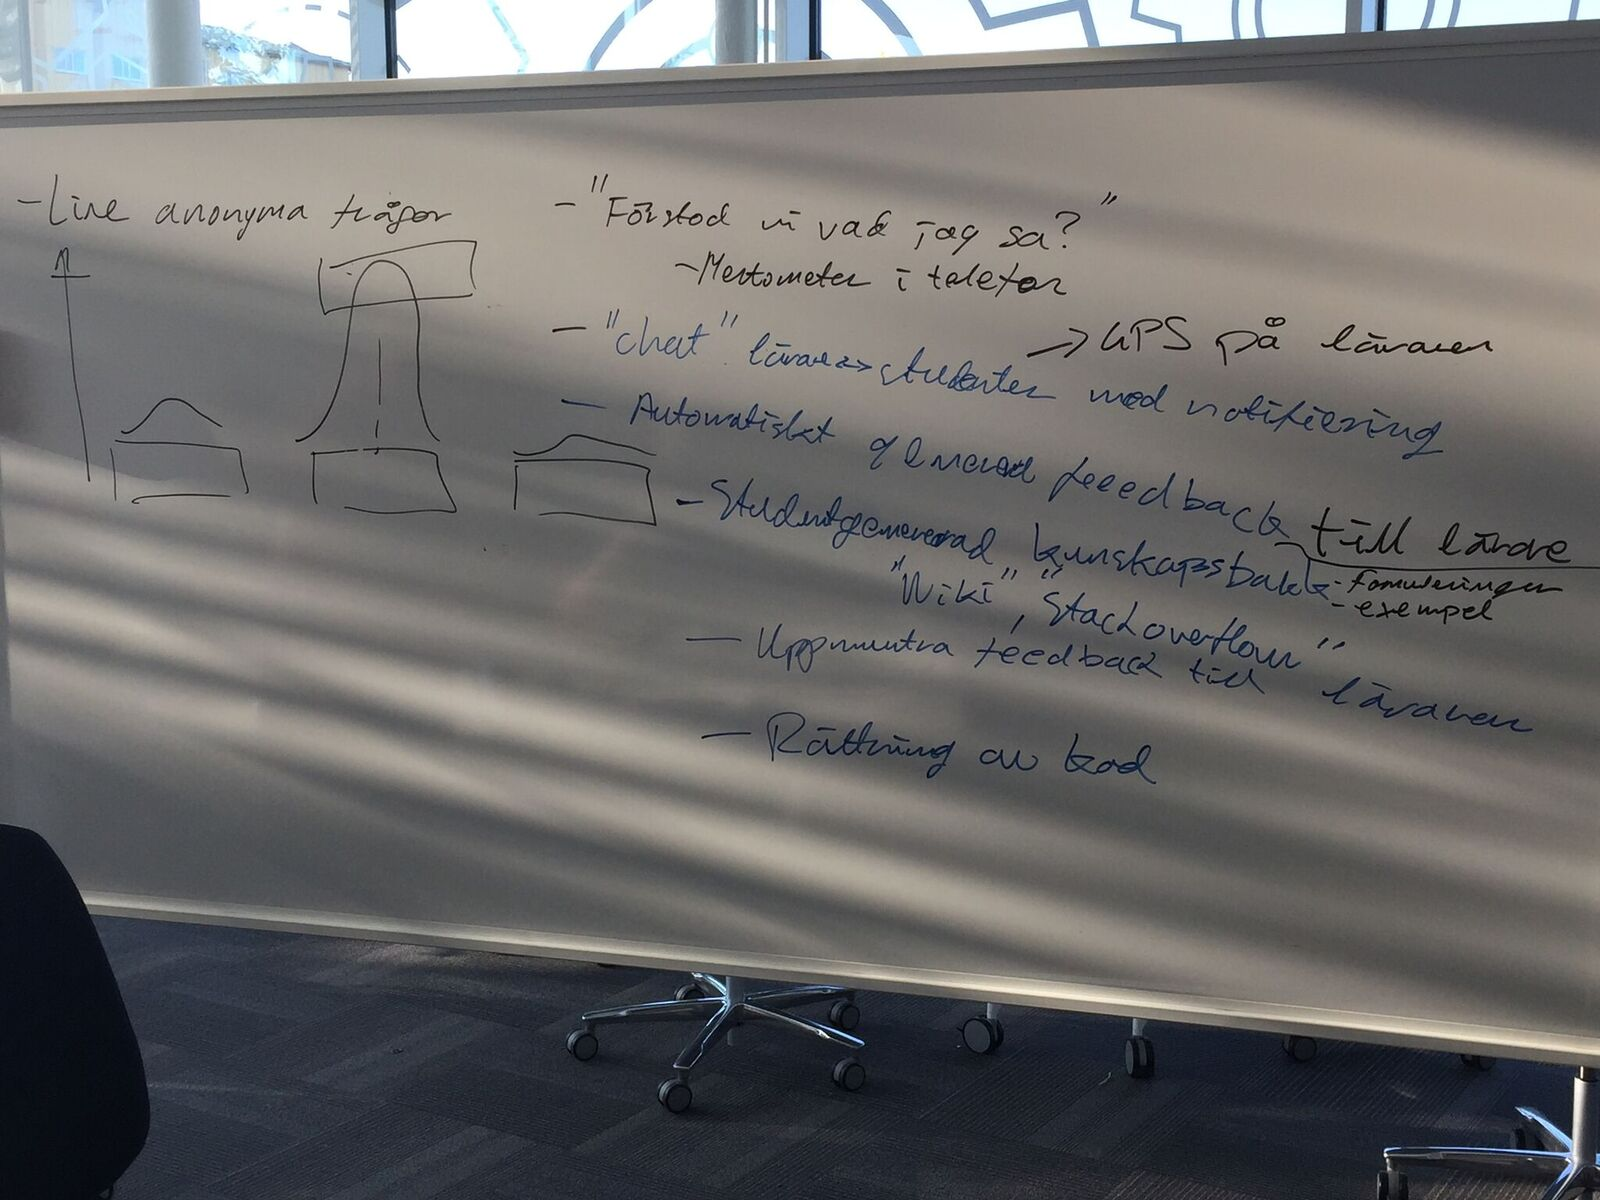
\includegraphics[width=\textwidth]{img/Grupp1_Workshop_mockup.jpg}
    \caption{A mockup over interface from workshop-group 1.}
  \end{minipage}
  \hfill
  \begin{minipage}[b]{0.7\textwidth}
      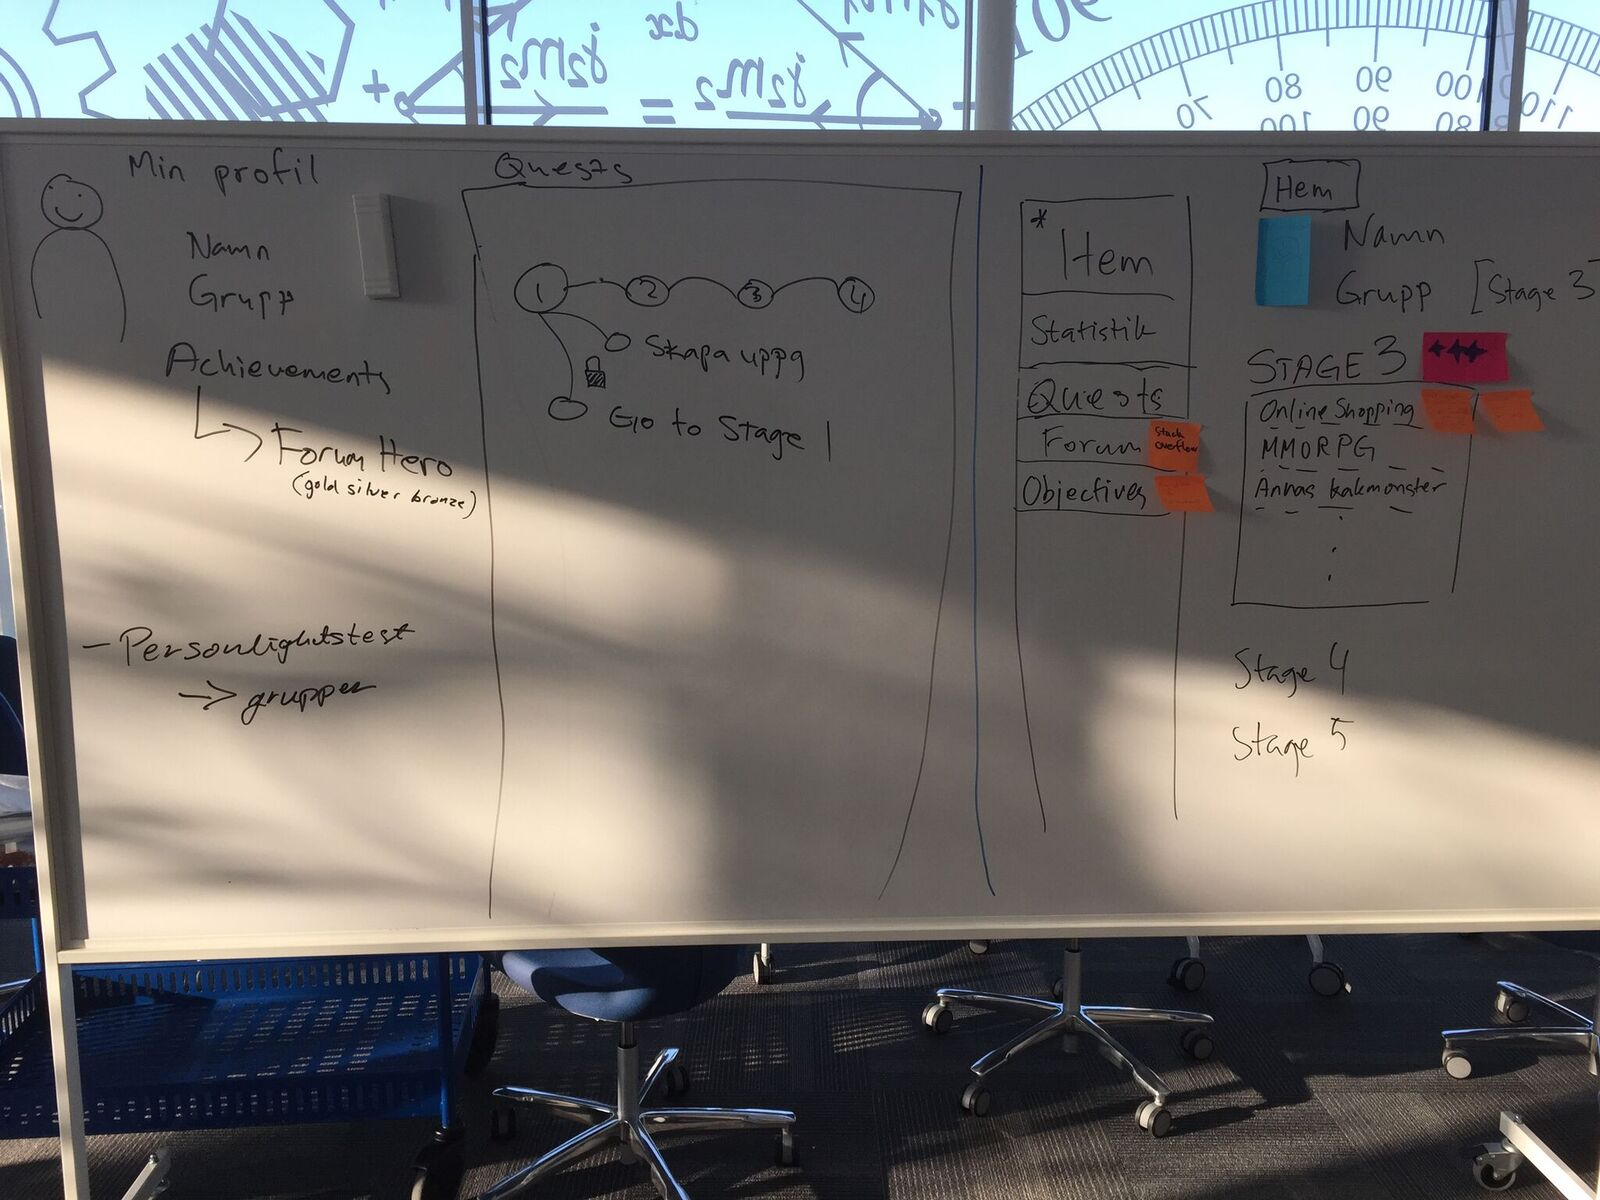
\includegraphics[width=\textwidth]{img/Grupp2_Workshop_mockup.jpg}
    \caption{A mockup over interface from workshop-group 2.}
  \end{minipage}
\end{figure}



\section{Design}
\subsection{Decisions} 
When the prestydy was completed it was time to make some decisions about the content of the platform, how it should look and how different parts should be implemented. To give a picture of how the design on the user interface should look like, a group sketched some simple mockups
so that every member could have the same starting point and vision. 

\begin{figure}[H]
  \centering
  \begin{minipage}[b]{0.7\textwidth}
    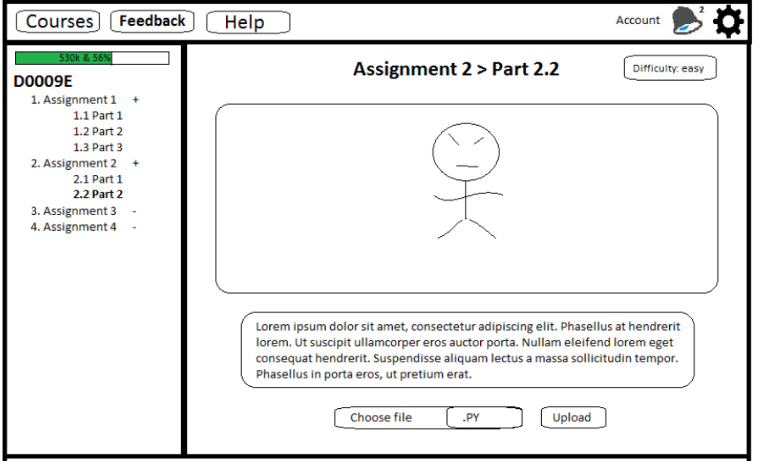
\includegraphics[width=\textwidth]{img/mockup1.png}
    \caption{An initial mockup over the assignment page.}
  \end{minipage}
  \hfill
  \begin{minipage}[b]{0.7\textwidth}
    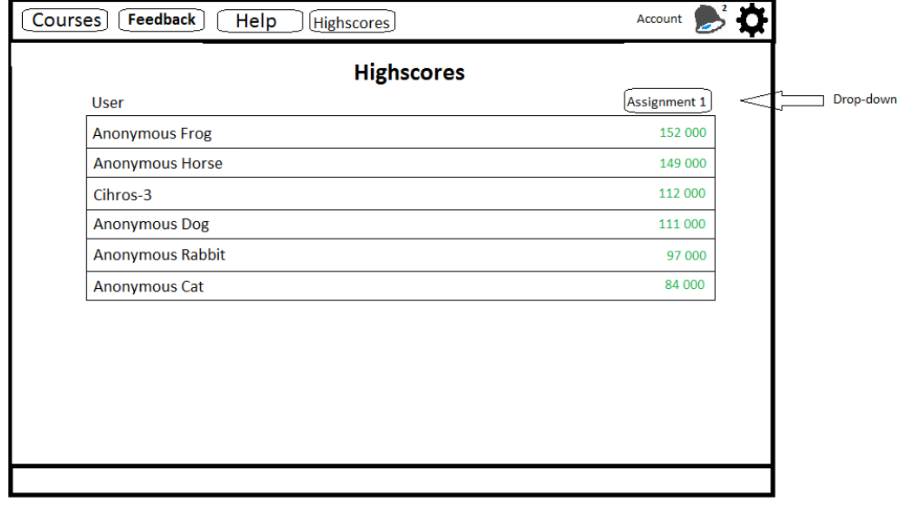
\includegraphics[width=\textwidth]{img/mockup2.png}
    \caption{An initial mockup over the leaderboard.}
  \end{minipage}
\end{figure}

The mockups were only used to have a base and the rest of the design would grown during the implementation time and it was mostly the frontend group that designed the pages. 
During the prestudy it become clear that the whole system flow was needed to be implemented. No one of the found an existing solution that would fit with the system and it couldn't be ensured that it will work over time. The system was divided into three parts. Tester whose main task was to implement a system that is able to test code that students write and send back some feedback. The frontend should implement the user interface and the gamification visualization. The backend is the in the middle and it will take the code from frontend and load a test from the database, send the submitted code along with the tests to Tester and then give the response (feedback) back to the frontend.

\begin{figure}[H]
\centering
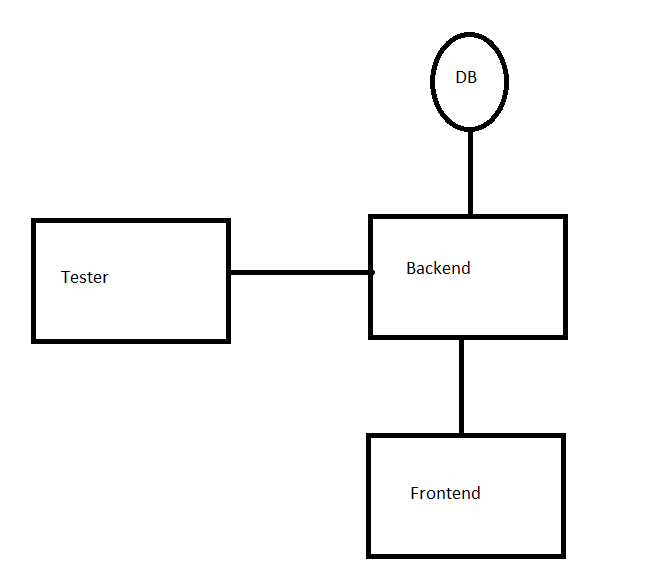
\includegraphics[scale=0.8]{img/SystemA.png}
\caption{A simple sketch over the system parts and how they are connected.}
\end{figure}

The time estimation for every separate part was difficult to estimate since the concept was fairly new for everyone. The decision of what programming language to use was based on the criteria, it should be fullstack meaning the same language should be used in every part so that if there is any interaction between the three groups it should be easy to understand the code. It should also be fairly modern programming language. The two alternatives was Python with frameworks or JavaScript with other frameworks. A democratic choice become JavaScript using Node.Js for backend and Tester, MongoDB as a NoSQL database and Angular4 for frontend. 


\subsection{Use-cases}
In the system there are two different roles, teacher and student. The teacher is able to create courses, assignments and invite students to the courses. The student can solve assignments.
Students who want to solve an assignment go to the site, log in, go to the specific assignment and write the code required in the assignment and submit it. The code is sent to the backend that saves the code to the database for future changes and loads the tests that belong to the assignment from the database. It then sends both the tests and the code to Tester which tests the code and sends back the output through the backend which in turn calculates the correct number of points that the student should be given for their solution. The output is now served to the frontend and the student can see if the code has passed or not with feedback.


\subsection{Frontend}
\begin{figure}[H]
\centering
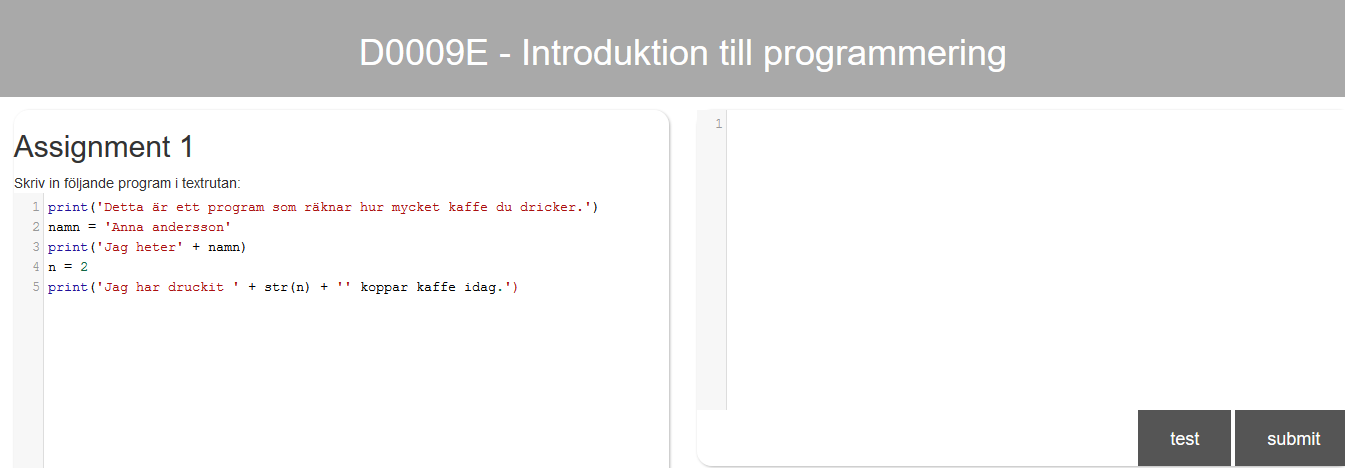
\includegraphics[scale=0.45]{img/Codemirror_pic.png}
\caption{A screenshot over how assignment looked when using codemirror.}
\end{figure}
\begin{figure}[H]
\centering
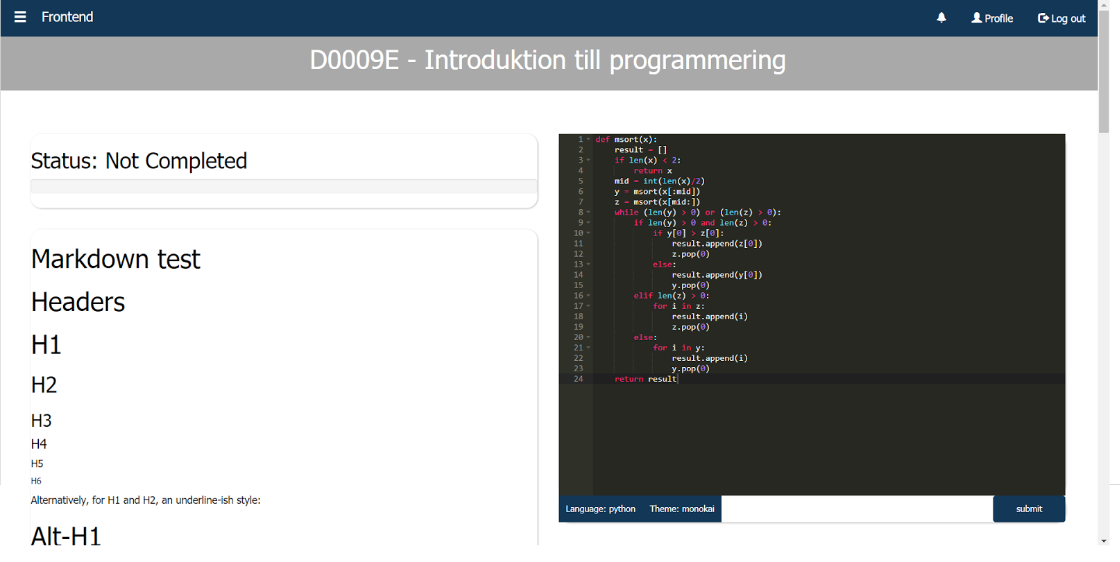
\includegraphics[scale=0.5]{img/Ace.png}
\caption{A screenshot over how assignment looked when using Ace. }
\end{figure}
\begin{figure}[H]
\centering
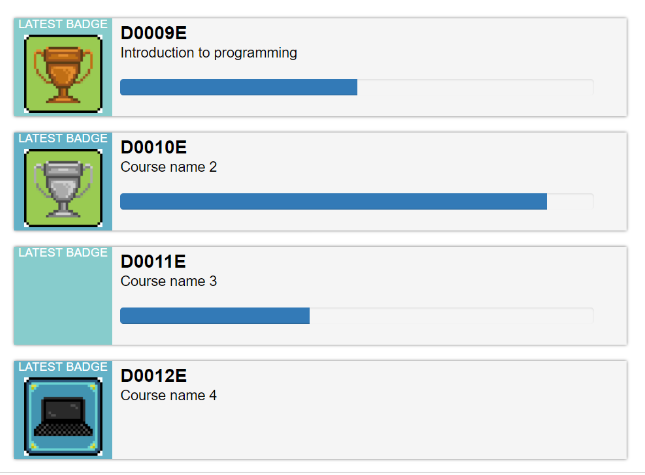
\includegraphics[scale=0.6]{img/Progress.png}
\caption{How the progress and badges look like.}
\end{figure}

\subsection{Backend}
A backend group was formed after all the prestudies were finished.
Beginning to work on the backend, the first decision that had to be made was what it was going to be developed in. Since it had been decided previously that the project would be a full-stack JavaScript solution the natural decision was to use node.js as server framework with express.js as a web framework to handle routing, for database it was decided to use the document database MongoDB.

The first few days were mostly spent on getting acquainted with node.js and its work flow.
After the group had gotten a general grasp of things, a coding standard was decided on and the group was divided into sub-parts in the backend.
The parts that the group was divided into were routes, database and continuous integration.
\\
It was decided that it was very important for continuous integration to be a part of the project. The reasoning for using continuous integration was that having a modern workflow where you could push changes to git and have them available on a live test server would be important to keep the project effective. Using continuous integration was also a good way to effectively separate production and development builds and a way to ensure that production builds always kept a certain standard and robustness.
However, while the idea and reasoning for using continuous integration was good, the concept wasn't put to as good use as it could have been. For the first half of the project, the continuous integration wasn't really used they way it was intended too, mainly due to communication errors and the fact that it wasn't needed as much, but for the second part of the project it was used more.

\subsection{Tester}

\section{Future work}
\subsection{Frontend}
\subsection{Backend}
\subsection{Tester}
\end{document}
